% Supplementary material for
%   "Machine Learning Surrogate Optimization Framework for Time-Based
%    Consolidation in Last Mile Parcel Delivery"
% Revision 1, 2026-08-28. Companion to tbc_preprint_main.tex.
%
% FIGURE SOURCES. Every figure below is produced by the revision scripts into
%   results/revision_2026_08_v6/figures/
% and is reached from here through the second \graphicspath entry, i.e. the
% relative path ../../results/revision_2026_08_v6/figures/. Once
% scripts/revision/71_sync_paper_figs.py has copied them into
% paper/EWGT_2026_rev1/figures/ under the same stems, the first entry wins and
% the relative path can be dropped. The stems are the supp_* names 70_ and 75_
% write; they are NOT renamed on sync.
%
% NUMBERS. All values come from grid v6 (results/revision_2026_08_v6/):
%   Section S1  -> _peek/discount_scenarios_v6.csv
%   Section S2  -> Kompendium 40.12/40.13 (label cost model term shares)
% Baseline of that grid: 1,898,091 EUR/wk routing, 2,098,401 EUR/wk operator.

\documentclass[11pt,a4paper]{article}

\usepackage[a4paper,left=2.5cm,right=2.5cm,top=2.5cm,bottom=2.5cm]{geometry}
\usepackage[utf8]{inputenc}
\usepackage[T1]{fontenc}
\usepackage{mathptmx}
\usepackage{amsmath}
\usepackage{amssymb}
\usepackage{eurosym}
\usepackage{graphicx}
\usepackage{booktabs}
\usepackage{caption}
\usepackage[colorlinks,linkcolor=blue,urlcolor=blue]{hyperref}

\graphicspath{{figures/}{../../results/revision_2026_08_v6/figures/}}

% S-numbering for everything
\renewcommand{\thesection}{S\arabic{section}}
\renewcommand{\thefigure}{S\arabic{figure}}
\renewcommand{\thetable}{S\arabic{table}}

\title{Supplementary material\\[2mm]
\large Machine Learning Surrogate Optimization Framework for Time-Based
Consolidation in Last Mile Parcel Delivery}
\author{L.\ Bienzeisler \and F.\ Petre \and O.\ Wage \and B.\ Friedrich}
\date{}

\begin{document}
\maketitle

This document collects the material referenced from the main text. All numbers
come from the same optimization grid as the main text and are taken against
that grid's own daily-delivery baseline ($1{,}898{,}091$~\euro\ per week in the
routing lens, $2{,}098{,}401$~\euro\ per week in the operator lens, summed depot
peak $1{,}239$ vehicles).

\section{Paying for the delay: a discount scenario}
\label{sec:supp_discount}

The service penalty $P$ steers the schedule search but is not a cash flow. It
is worth asking what remains if the operator actually pays customers for
waiting. We evaluated two payout rules on the same grid, for both plans and
both lenses: (a) $P$~\euro\ per parcel and waiting day, that is, the steering
penalty turned into a real payment; and (b) a flat $0.50$~\euro\ per delayed
parcel, independent of how long it waits. A parcel counts as delayed if it
arrives on a non-delivery day of its cell and its recipient is willing to wait.
The count is taken from the realized demand on the skipped days rather than
from an even weekday split, because the optimized patterns preferentially skip
days of below-average demand; the even-split approximation understates the
delayed volume by up to $5\%$ at $P = 1$ and would inflate the break-even
discount accordingly.

At full adoption and under the operator-polished plan, $679$ thousand of the
$1.26$~million weekly parcels are delayed at $P = 0$, falling to $405$, $237$,
$153$ and $109$ thousand at $P = 0.25$, $0.5$, $0.75$ and $1$.
Table~\ref{tab:supp_discount} gives the net saving after payout under both
rules and in both lenses, together with the break-even discount.

\begin{table}[h]
  \centering
  \caption{Net saving after paying the delay out, operator-polished plan at
  $\theta = 1$. Rule (a): $P$~\euro\ per parcel and waiting day. Rule (b): a
  flat $0.50$~\euro\ per delayed parcel. Break-even is the largest flat
  discount per delayed parcel at which the schedule still matches daily
  delivery.}
  \label{tab:supp_discount}
  \small
  \begin{tabular}{l rrrrr}
    \toprule
    $P$ (\euro/p/d) & $0$ & $0.25$ & $0.5$ & $0.75$ & $1$ \\
    \midrule
    Delayed parcels (thousand/wk)      & $679$ & $405$ & $237$ & $153$ & $109$ \\
    \addlinespace
    Rule (a), operator lens (\%)       & $24.3$ & $16.6$ & $11.2$ & $8.1$ & $6.1$ \\
    Rule (a), routing lens (\%)        & $20.0$ & $10.2$ & $5.1$  & $2.4$ & $0.8$ \\
    \addlinespace
    Rule (b), operator lens (\%)       & $8.1$ & $\mathbf{12.9}$ & $12.1$ & $10.4$ & $9.1$ \\
    Rule (b), routing lens (\%)        & $2.1$ & $\mathbf{6.1}$  & $6.0$  & $5.0$  & $4.1$ \\
    \addlinespace
    Break-even discount, operator (\euro) & $0.75$ & $1.17$ & $1.57$ & $1.93$ & $2.25$ \\
    Break-even discount, routing (\euro)  & $0.56$ & $0.78$ & $0.98$ & $1.12$ & $1.21$ \\
    \bottomrule
  \end{tabular}
\end{table}

Three readings follow. First, under rule~(a) the saving is roughly halved from
$P = 0.25$ onwards but never eliminated: the penalty is a transfer, not a
destruction of value. Second, under the flat rule~(b) the ordering of the
operating points changes, because $P = 0$ delays too many parcels to be worth
its larger gross saving. In the operator lens $P = 0.25$ becomes the best point
on the grid, ahead of $P = 0.5$ by $0.8$~pp. In the routing lens the two are
$6.052$ and $6.043\%$, i.e.\ $0.01$~pp apart; that is a tie at the resolution
of this grid, and considerably smaller than the surrogate's own bias, so the
routing lens should not be read as preferring either. Third, the break-even
discount rises with $P$ and exceeds the $50$ cents assumed here everywhere, so
a real discount programme of that size is affordable at every operating point.

At partial adoption the discount decides which lens stays positive. At
$P = 0.25$ and $\theta < 1$, rule~(b) leaves the routing lens between $+0.1$
and $-2.1\%$ --- that is, at or below break-even --- while the operator lens
holds between $+3.4$ and $+6.2\%$. Under partial adoption a discount programme
is therefore only defensible under weekly staffing.

\section{The labour double count in the label cost model}
\label{sec:supp_labour}

Every solver label, and therefore every predicted, baseline and validated cost
in this study, follows the effective cost model $189.15$~\euro\ per vehicle and
day, $0.3864$~\euro\ per kilometre and $36$~\euro\ per route-hour, the last
because the solver's default per-hour rate was active when the labels were
generated. The three terms contribute $72.2$, $6.0$ and $21.7\%$ of label cost.
The driver's wage is part of the fixed daily cost, and the route-time charge is
separate and additional, so driver labour is charged twice.

The consequence is confined to levels. Baseline, scenarios, prediction and
out-of-sample validation all carry the term, so every comparison in the paper is
internally consistent and the relative savings are unaffected; route time is
dominated by per-parcel service time, which barely moves between daily and
batched operation, so a near-constant term sits in numerator and denominator
alike and damps rather than inflates the reported percentages. Absolute cost
levels do contain it: about a fifth of every level reported here, in either
lens, is this double-counted term. Re-labelling the training pool with the
per-hour rate set to zero, and re-training on it, is left to future work; it
would lower the levels without materially changing the comparisons made here.

\section{Supplementary figures}
\label{sec:supp_figures}

\begin{figure}[h]
  \centering
  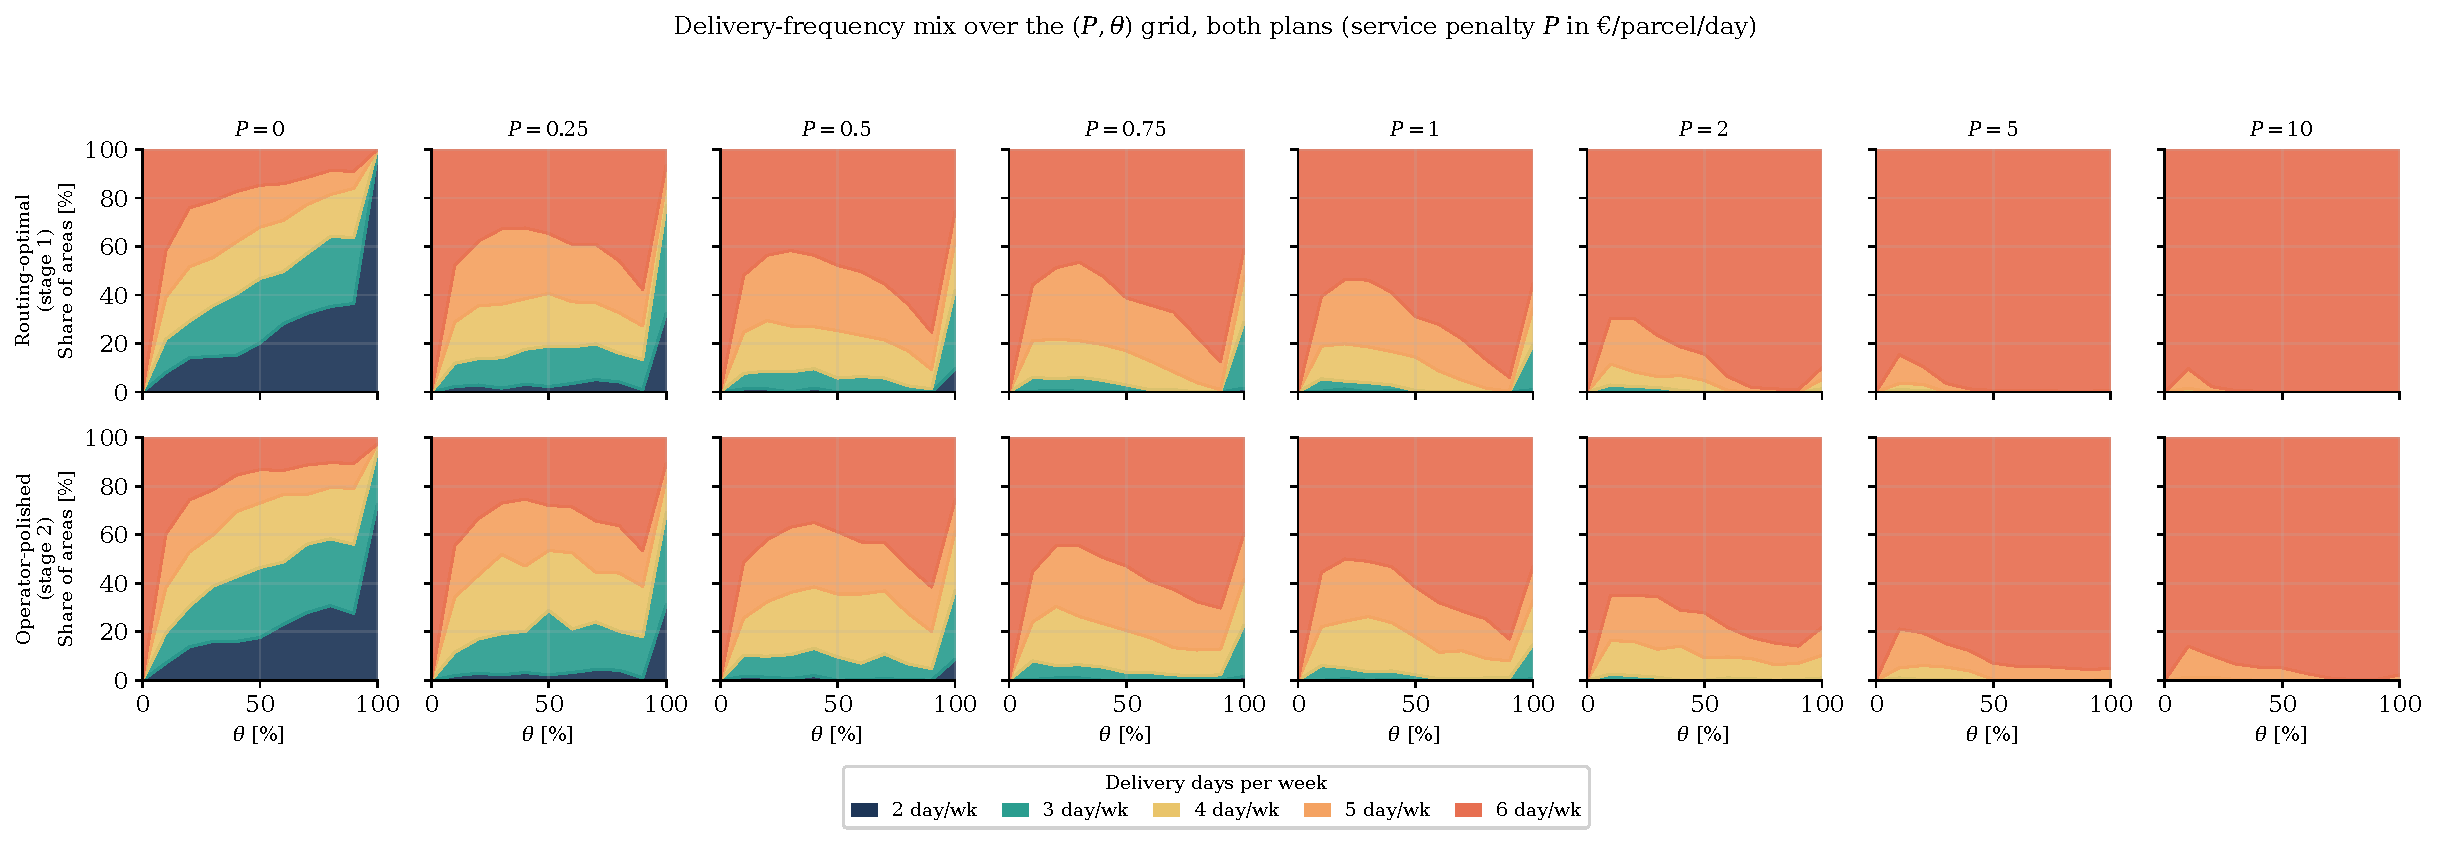
\includegraphics[width=\linewidth]{supp_fig4_freq_mix_two_plans.pdf}
  \caption{Delivery-frequency mix across the $312$ cells for both plans: the
  routing-optimal plan of stage~1 (upper row) and the operator-polished plan of
  stage~2 (lower row), one column per service penalty $P$. The two plans differ
  in delivery frequency and not only in weekday placement, so the rows are not
  two views of one schedule; the delivery-day count differs in $20.1\%$ of the
  $27{,}456$ cell--grid-point pairs. Figure~4 of the main text shows the upper
  row.}
  \label{fig:supp_mix_two_plans}
\end{figure}

\begin{figure}[h]
  \centering
  \includegraphics[width=\linewidth]{supp_fig4b_mean_days.pdf}
  \caption{Mean weekly delivery frequency $\bar{f}$ of both plans over the
  $(P, \theta)$ grid. The non-monotonicity in $\theta$ around
  $\theta = 0.8$--$0.9$ is the express-residual effect discussed in the main
  text: the service penalty scales with $\theta$ while the residual volume that
  a skipped delivery day leaves behind becomes too thin to fill a vehicle.}
  \label{fig:supp_mean_days}
\end{figure}

\begin{figure}[h]
  \centering
  \includegraphics[width=\linewidth]{supp_fig5_grid_heatmap_v2.pdf}
  \caption{The $(P, \theta)$ grid in both cost lenses. Figure~5 of the main
  text reports all six panels in the routing lens; this version adds the
  operator lens, in which a vehicle-day below its depot's weekly peak carries
  only variable cost.}
  \label{fig:supp_grid_two_lens}
\end{figure}

\begin{figure}[h]
  \centering
  \includegraphics[width=\linewidth]{supp_fig5b_offdiagonal_v2.pdf}
  \caption{The two off-diagonal lens--plan combinations that Figure~5 of the
  main text does not show: the operator-lens outcome of the routing-optimal
  plan, which is negative over much of the grid, and the routing-lens outcome
  of the operator-polished plan.}
  \label{fig:supp_offdiagonal}
\end{figure}

\begin{figure}[h]
  \centering
  \includegraphics[width=\linewidth]{supp_fig6_structural_v2.pdf}
  \caption{Per-cell structural breakdown of the saving in euro, by carrier
  class, region type, hub distance, postal-code area size and parcels per
  drop-site. Figure~6 of the main text shows the same breakdown as a
  percentage.}
  \label{fig:supp_structural}
\end{figure}

\begin{figure}[h]
  \centering
  \includegraphics[width=\linewidth]{supp_fig6b_operator_lens_v2.pdf}
  \caption{The operator lens per depot: per-LSP knee $P^\star$ in both lenses,
  and the per-depot operator saving and delivery frequency by depot size in
  cells served ($1$, $2$--$4$, $5$--$12$, $\geq 13$). The buckets below $13$
  cells consist exclusively of DHL depots, because each of the other six
  providers serves the region from a single depot; the single-cell half of the
  rotation mechanism is therefore a within-DHL result and not a general law.}
  \label{fig:supp_operator_lens}
\end{figure}

\begin{figure}[h]
  \centering
  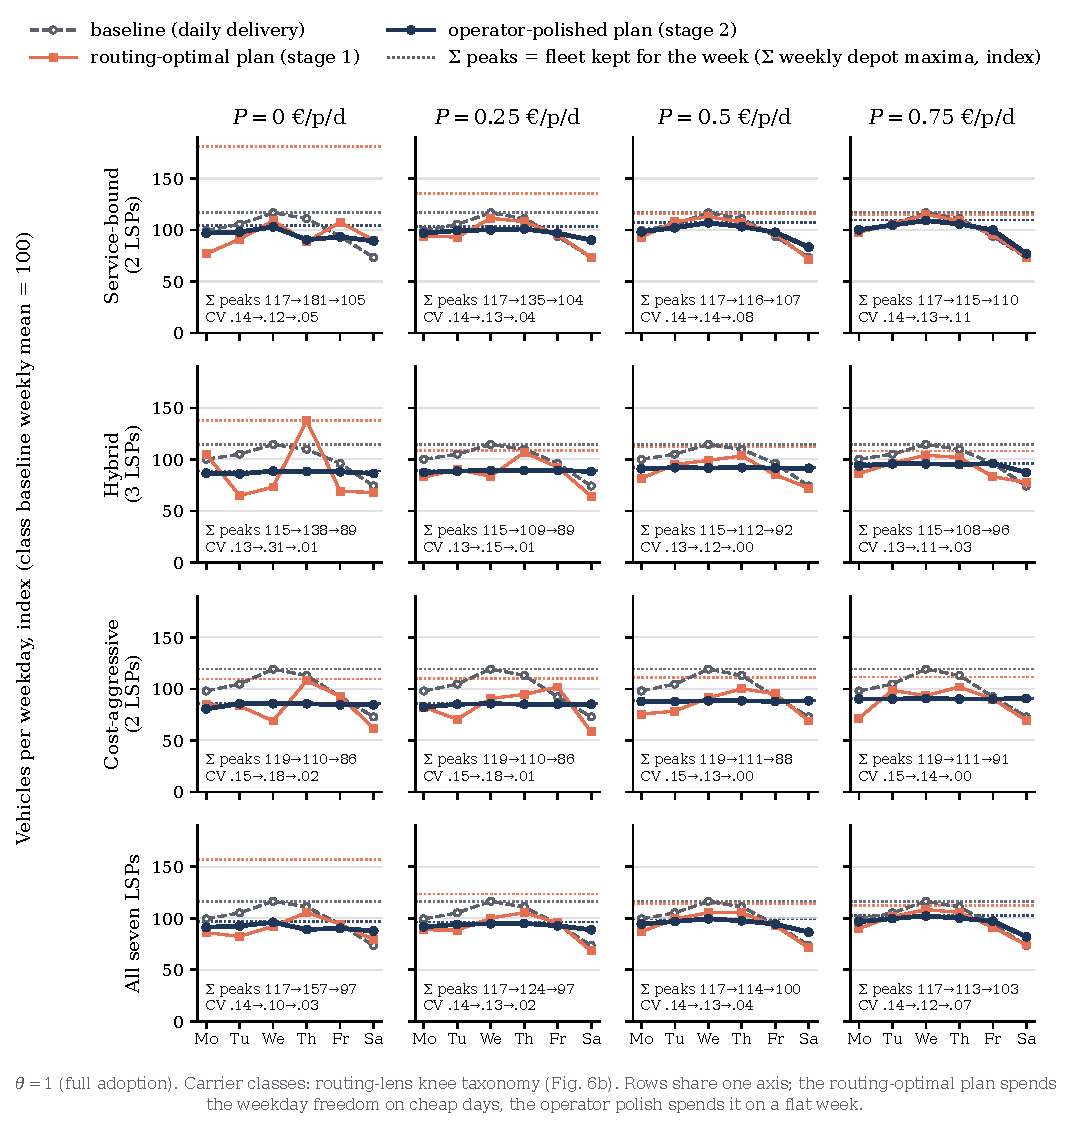
\includegraphics[width=\linewidth]{supp_fig7_fleet_week_classes.pdf}
  \caption{Weekly fleet profile by carrier class and plan, indexed on each
  class's baseline weekly mean. Temporal consolidation creates the freedom to
  move a delivery day but does not level the week by itself: the
  routing-optimal plan raises the summed depot peak, and only the operator
  polish converts the freedom into a flatter profile.}
  \label{fig:supp_fleet_week}
\end{figure}

\begin{figure}[h]
  \centering
  \includegraphics[width=\linewidth]{supp_map_saving_P_v2.pdf}
  \caption{Cost saving per postal-code area at full adoption for the
  operator-polished plan, in the routing lens, over the service penalty $P$.
  System saving $20.0$, $16.7$, $12.3$, $9.0$, $6.9$ and $2.2\%$ at
  $P = 0$, $0.25$, $0.5$, $0.75$, $1$ and $2$; at $P = 0$ the areas span
  $6.0$ to $29.4\%$ around a median of $20.5\%$.}
  \label{fig:supp_map_saving}
\end{figure}

\begin{figure}[h]
  \centering
  \includegraphics[width=\linewidth]{supp_penalty_raumtyp_v2.pdf}
  \caption{Saving against the service penalty by region type at full adoption,
  euro-weighted, for the operator-polished plan in the routing lens: rural
  $23.2$, suburban $18.9$ and urban $15.6\%$ at $P = 0$, converging to at most
  $0.7\%$ from $P = 5$ onwards.}
  \label{fig:supp_penalty_raumtyp}
\end{figure}

\begin{figure}[h]
  \centering
  \includegraphics[width=\linewidth]{supp_map_freq_theta_v2.pdf}
  \caption{Parcel-weighted median weekly delivery frequency per postal-code
  area at $P = 0.25$, over the willingness-to-wait share $\theta$, for the
  operator-polished plan. Three delivery days per week dominate at full
  adoption, with a two-day cluster in the south of the region.}
  \label{fig:supp_map_freq}
\end{figure}

\begin{figure}[h]
  \centering
  \includegraphics[width=\linewidth]{supp_map_wait_theta_v2.pdf}
  \caption{Parcel-weighted mean additional wait of a held parcel per
  postal-code area at $P = 0.25$, over $\theta$, for the operator-polished
  plan. The maximum area value is $0.7$ days at full adoption.}
  \label{fig:supp_map_wait}
\end{figure}

\end{document}
